
%Mu2e Overview

\label{cl:sec:mu2e}

The Mu2e experiment, to be hosted at Fermilab, is a flagship component
of the U.S.\ Intensity Frontier program~\cite{IF_review} and will
search for the charged-lepton-flavor-violating process of coherent
muon-to-electron conversion in the presence of a nucleus ($\mu^-N
\rightarrow e^-N$).  The Mu2e experiment will improve sensitivity
compared to current experimental by four orders of
magnitude~\cite{Mu2eCDR} and will set a limit on $R_{\mu e}$, defined
as,

%
\begin{eqnarray}
  R_{\mu e} &=& \frac
  {\Gamma(\mu^{-}\;  N(A,Z) \to e^{-}\; N(A,Z)}  {\Gamma(\mu^{-}\; N(A,Z)\to \nu_{\mu}\; N(A,Z-1))},\end{eqnarray}
%

where $N(A,Z)$ denotes a nucleus with mass number $A$ and atomic
number $Z$.  The numerator corresponds to the rate for the CLFV
conversion process and the denominator corresponds to the rate for
ordinary muon capture on the same nucleus.  The current best limit is
$R_{\mu{}e}<7\times10^{-13}$\cite{Bertl:2006up}.

There is no observable Standard Model contribution to the $\mu^-N
\rightarrow e^-N$ signal at Mu2e.  Neutrino oscillations imply that
muon-to-electron conversion can proceed via a penguin diagram that
contains a $W$ and an oscillating neutrino. However, the rate for this
conversion process is more than 30 orders of magnitude below the
projected sensitivity of the Mu2e experiment.  Any signal observed at
Mu2e would be an unambiguous indication of new
physics~\cite{Marciano:2008zz,deGouvea:2013zba}.

The approach of the Mu2e experiment is to stop low-momentum muons from
a pulsed beam on an aluminum target to form muonic atoms and then to
measure the resulting electron spectrum.  The signal would produce a
mono-energetic electron with an energy of about 105~MeV.  In order to
reach the design sensitivity (single-event sensitivity of $2\times
10^{-17}$), about $10^{18}$ muons must be stopped.  Keeping the
background expectation to less than one event in this high-intensity
experiment is obviously quite a challenge and results in the unique
experimental setup summarized below and depicted in
Fig.~\ref{cl:fig:mu2e}.

The first step in the experiment is to produce the low-momentum pulsed
muon beam.  Recycled Tevatron infrastructure will deliver 8~GeV
protons with 1695~ns bunch spacing to the experiment.  The 1695~ns
revolution period of the Debuncher ring is well suited for the Mu2e
experiment given that the lifetime of the muonic aluminum is about
864~ns.  Pions and muons produced inside the production solenoid are
collected and passed to the S-shaped muon beamline where absorbers and
collimators are optimized to eliminate positively-charged particles
and anti-protons while efficiently transmitting low-energy
negatively-charge pions and muons.  Most of the pions will decay
inside the 13~m long beamline, while about 40\% of surviving muons
will be stopped in an aluminum stopping target.  Simulations estimate
that Mu2e will produce $0.0016$ stopped muons per proton on target.



\begin{figure}
\centering
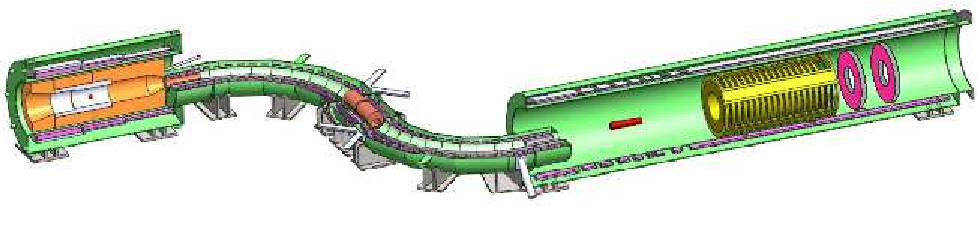
\includegraphics[width=0.8\textwidth]{ChargedLeptons/Figures/mu2edisk_scaled.pdf}
\caption{The Mu2e experimental setup. The pulsed proton beam enters
the production solenoid (far left) from the top right.  The muons
produced are captured by the production solenoid and transported
through the S-shaped transport solenoid to the aluminum stopping
target (small red cylinder).  Electrons produced in the stopping
target are captured by the magnetic field of the detector solenoid
(right) and transported through the tracker (yellow) where the
momentum is measured.  The electrons then strike the electromagnetic
calorimeter (pink annuli), which provides an independent measurement.
A cosmic-ray-veto system and some other parts of the apparatus are not
shown.
}
\label{cl:fig:mu2e}
\end{figure}



Muons stop in the target and form a muonic atom.  As they settle into
the K-shell a cascade of X-rays will be emitted.  By detecting these
X-rays the rate of stopped muons can be measured, thereby establishing
the denominator of $R_{\mu e}$. About 60\% of stopped muons will
undergo muon capture on the nucleus while the other 40\% will decay in
orbit (DIO).  The DIO process produces an electron with a continuous
Michel distribution including a long tail due to photon exchange with
the nucleus.  In the limit where the neutrinos carry no energy from
the Michel decay, the electron carries the maximum energy of 105~MeV~\cite{czarnecki}.
In this limit, the DIO electron is indistinguishable from the $\mu^-N
\rightarrow e^-N$ conversion signal.  In addition, mis-measurements of
the DIO electron momentum contributes to an irreducible background.
In order to combat the DIO background, the Mu2e experiment requires a
tracking detector with momentum resolution of about $0.1$\%.


 
To accomplish the required momentum resolution, the Mu2e tracker will
use straw tubes in vacuum.  The inner radius of the tracker is empty
so that only tracks with transverse momenta above $53$~MeV/c will pass
through any of the straw tubes. The Mu2e scintillating-crystal (LYSO)
calorimeter will provide cross checks of signal candidates and
particle identification.  The calorimeter also has an empty inner-radius 
region.  The empty inner regions effectively make the tracker
and calorimeter blind to the bulk of the DIO electrons and muons that
don't stop in the target and allow these detectors to handle the
high-intensity environment required for the experiment.


The primary backgrounds for the Mu2e experiment can be classified into
several categories: intrinsic muon-induced back grounds, late-arriving
backgrounds, and miscellaneous backgrounds, primarily anti-proton
induced and cosmic-ray induced backgrounds. The moun induced
backgrounds arise from muon DIO and radiative muon capture.  The
kinematic endpoint of the electron energy distribution is slightly
below 105 MeV, so this background, like the DIO, can be mitigated by
minimizing non-Gaussian contributions to the tails of the momentum
resolution.  The dominant late-arriving background arises from
radiative pion capture and subsequent conversion of the $\gamma$ in
the stopping target material to produce a 105~MeV electron.
Late-arriving backgrounds like this can be controlled by taking
advantage of the long muon lifetime and by optimizing the properties
of the pulsed beam.  After a beam pulse there is a delay of about
700~ns before the signal timing window begins.  In order to avoid
late-arriving backgrounds in the signal time window Mu2e requires the
fraction of protons outside the beam pulse to be less than $10^{-10}$,
which will be achieved and monitored with dedicated systems.  Beam
electrons, muon decay in flight, and pion decay in flight are other
late-arriving backgrounds that are defeated through the combination of
the pulsed beam and delayed signal window.



Cosmic-ray muons may interact within the detector solenoid region and
produce background electrons.  Passive shielding and an active
cosmic-ray-veto system are employed to ensure that cosmic rays are a
sub-dominant background.
 


The total background expectation in the Mu2e experiment for a
three-year run at 8~kW beam power is less than 0.5 events and
summarized in Table~\ref{cl:tab:PXBgd}.

%\begin{table}[t]
%  \centering
%  \begin{tabular}{llcr} \hline\hline
%    Category      
%         & Source    &\hspace{0.15in}   & Events \\ \hline
%    \multirow{2}{*}{Muon-induced}    
%         & $\mu$ decay in orbit       & & 0.22   \\ 
%         & radiative $\mu$ capture    & & $<0.01$  \\ \hline
%    \multirow{4}{*}{Late arriving}
%         & radiative $\pi$ capture    & & 0.03   \\
%         & beam electrons             & & $<0.01$  \\
%         & $\mu$ decay in flight      & & 0.01   \\
%         & $\pi$ decay in flight      & & $<0.01$  \\ \hline
%    \multirow{3}{*}{Miscellaneous}              
%         & anti-proton induced        & & 0.10   \\
%         & cosmic-ray induced         & & 0.05   \\
%         & pat. recognition errors    & & $<0.01$  \\ \hline
%    Total Background 
%         &                            & & 0.41   \\ \hline\hline
%  \end{tabular}
%  \caption{A summary of the current Mu2e background estimates.
%  }
%  \label{cl:tab:Mu2eBackgrounds}
%\end{table}

